% don't remove the folling lines, and edit the defintion of \main if needed
\documentclass[../report.tex]{subfiles}
\providecommand{\main}{..}
\IfEq{\jobname}{\currfilebase}{\AtEndDocument{\biblio}}{}
% until here

\begin{document}
% this is the extra information to be used for the general sections.
\section{DM and Dark Sectors at beam dump and fixed target experiments}

In this section we  summarize the physics case for $\sim$ few keV--GeV scale dark matter and other hidden sector particles and identify key targets of opportunity for future experimental efforts. 
%This summary is based on the discussions at the Granada Open Symposium on the Update of the European Strategy for Particle Physics as well as the relevant community input documents [ID9] 9, 11,12, 28, 36, 42, 75, 94,102, 129, 131, 153) submitted to this process. 
%Our discussion also benefits from the more detailed reports~\cite{BRN report}.


\subsection{Theoretical Motivation}
%There is a compelling case to search for thermal Dark Matter with a mass in the keV - 100 TeV range. In this range, theoretical models become highly predictive as they do not depend on assumptions about unknown cosmological epochs such as inflation or baryogenesis.
The lighter half of the thermal dark matter  mass range, few keV--GeV, is currently underexplored and typically inaccessible using traditional WIMP detection strategies \cite{Battaglieri:2017aum}; new techniques are necessary to comprehensively probe the predictive models in this window.
%If the DM-SM interaction rate ever exceeded the Hubble expansion rate in the early universe, the DM abundance is set by the strength of the DM-SM annihilation rate independently of any assumptions about unknown cosmological epochs (e.g. inflation or baryogenesis). Such a predictive, thermal origin is only compatible with DM masses between $\sim$ few keV-100 and the lighter half of this mass range (few keV - GeV) is currently underexplored and typically inaccessible using traditional WIMP detection strategies ; new techniques are necessary to comprehensively probe the predictive models in this window. 
There are several key differences between traditional WIMPs and sub-GeV light DM (LDM) candidates. Unlike WIMPs, which can carry electroweak charge, LDM must be neutral under all SM gauge interactions -- otherwise it would have been discovered at LEP.\footnote{If $<$ GeV  DM were electrically millicharged, the size of the coupling necessary to avoid cosmological  overproduction is excluded by a variety of experiments \cite{Davidson:2000hf,Berlin:2018sjs}; additional forces are still necessary even if light DM is also millicharged.}
Furthermore, under the assumption of standard cosmology, in order to achieve the observed relic density for LDM particles, such models require couplings to the SM sector that are much larger than $G_{\rm F}$ \cite{Lee:1977ua}. This implies the existence of a light, %new force-carrier 
mediator between the SM and a new dark sector. If the mediators 
%connecting to SM particles through portals, 
are produced on-shell in the laboratory, they can decay either to LDM or to SM particles through the  portal couplings (see Sect.~\ref{sec:BSM-FIPs} for a summary). Improving experimental sensitivity to both LDM and SM decay channels has important implications for different theoretical scenarios.

No single experiment or approach is sufficient to cover the vast parameter space that dark sectors 
can occupy \cite{Izaguirre:2015yja,Battaglieri:2017aum}. A comprehensive dark sector program therefore relies on a complementary set of experiments and techniques that span the multitude of dark sector signatures and collectively cover the broad mass and coupling range:

\vspace{- 1mm}
{\bf Mediators decaying to LDM:} The most predictive class of thermal LDM models involves mediators that are heavier than  (twice) the LDM candidate and, therefore, decay to LDM pairs when produced on shell. Because the mediator is heavier than the LDM, the only kinematically accessible annihilation\footnote{When DM and mediator masses
are nearly degenerate, ``forbidden'' dark matter \cite{DAgnolo:2015ujb} 
serves as a notable counterexample to this claim.} channel for  early-Universe freeze-out is the $s$-channel {\it DM~DM~$\rightarrow$ SM SM} reaction which depends on the mediator's coupling to both dark and visible matter. 
%(see Fig. X in the supplement). 
Thus, the SM-mediator coupling occuring through a portal,  must have a minimum value to realize a thermal annihilation cross section, so mediators that decay to LDM feature predictive experimental-sensitivity targets; improving coverage to such mediators by 2--3 orders of magnitude in cross section can convincingly discover or falsify a broad class of thermal DM candidates whose relic density arise from annihilation directly into SM particles in the early Universe \cite{Battaglieri:2017aum,Izaguirre:2015yja}. 

\vspace{- 1mm}
{\bf Mediators decaying to SM particles:} If the mediator is {\it lighter} than the thermal LDM candidate, freeze-out occurs through {\it DM DM $\rightarrow$ mediator mediator} annihilation reactions, 
%(see Fig X' in supplement), 
which are independent of the SM-mediator coupling. In this regime, the mediator decays  to SM particles and motivates searches for new forces. However, in the event of a discovery, there is no necessary connection to thermal LDM; new particles with SM decays can exist independently of any DM assumptions. Indeed, beyond the thermal DM motivation, such particles arise in various new physics scenarios related to  leptogenesis, electroweak baryogenesis, %\cite{Carena:2018cjh}, 
the electroweak hierarchy problem, neutrino mass generation,
(see BSM chapter), and non-thermal DM scenarios which do not feature predictive experimental sensitivity targets, but are nonetheless well-motivated theoretically.
In many of these other scenarios, the SM coupling is required to be very small, so if the mediator is a long-lived particle (LLP), it can decay at a macroscopic distance, away from its production point, in an accelerator-based experiment.  
%which  decays a macroscopic distance away from its production point in an accelerator-based experiment. 
\subsection{Experimental techniques}
As the mediators of the dark sector couple weakly to the SM, facilities with high energy and intensity beams impinging on dense targets are essential in order to maximize the experimental sensitivity to such models. Facilities at CERN's SPS or SLAC's LCLS-II, will have unprecedented sensitivity to a wide range of dark sector models and offer unique opportunities to explore large portions of the relevant parameter space. The two main experimental techniques are beam-dump and fixed-target missing-energy/momentum searches. \\


\noindent {\bf Beam dump:} 
A high-intensity beam of relativistic particles (electrons, protons or muons) impinges on a thick, passive target. The detector, consisting of spectrometers and calorimeter systems are installed  10s--100s of meters downstream of the target. Shielding is placed between the target and detector to absorb SM particles. Signal candidates are reconstructed through electromagnetic energy depositions in the detector in time-coincidence with beam bunches.
%A signal consists of any electromagnetic energy deposited in the detector in time-coincidence with the beam bunches. 
If dark sector mediators are produced in the target (eg. via meson decays,  Drell-Yan or bremsstrahlung), a beam-dump signal can arise in two main ways:

1) If the mediator decays to LDM particles, the LDM can pass through the shielding material, enter the detector, and scatter off detector atoms, whose relativistic recoils are detectable \cite{deNiverville:2011it,Izaguirre:2013uxa}. %(see Fig X in supplement). 
This search strategy is akin to direct detection with two important differences a) the DM is produced directly at the target (not from the halo) and  b) the DM is relativistic, so even light particle masses ($\ll$GeV) can induce highly energetic target-particle recoils well above detection thresholds. Since mediator production  and the LDM scattering both scale as the SM-mediator coupling squared, this signal is proportional to the fourth power of this coupling.

2) If, instead, the mediator decays to SM particles, beam-dump signals arise from the decay products of a Long-Lived mediator Particle (LLP) that decays in between the shielding and the end downstream spectrometer. In this scenario, the signal rate depends on both mediator production (which scales as the SM-mediator coupling squared) and on its decay probability in the region of interest (which is also proportional to the SM-mediator coupling squared), so in total, this signal is proportional to the fourth power of the mediator-SM coupling. 
%Figure \ref{LLP} shows some the parameter space for representative LLP scenarios involving dark scalars (Higgs portal), fermions (HLN), annd axion like particles (ALPs).
%%%% REPETITION OF ABOVE %%%%%
%We note that in both cases, the signal at a beam dump is very similar (electromagnetic energy is deposited inside the detector) and the signal rate scales as the fourth power of the SM-mediator coupling. 

The SHiP experiment~\cite{Anelli:2015pba,Alekhin:2015byh} is an example of a beam dump experiment with a dual spectrometer to search for scenarios 1) and 2) simultaneously.
%%%%%%% COMMENT %%%%%%
% i) NA62 and KLEVER do not exactly fall into this category now and will mention them later
% ii) REDTOP is not quite what we describe above given that it has no shieling (target is thin strips of material surrounded by hermetic detector...)

\noindent {\bf Missing-energy/momentum} In this setup, a relativistic beam of particles (electrons or muons) also strikes a fixed-target, but the energy of each beam particle is measured both before and after it passes through the target. If the beam particle scatters inside the target and produces a new mediator which decays to LDM, the beam particle typically emerges with a much lower energy and there is no other SM particle production detected \cite{Izaguirre:2014bca,Banerjee:2016tad,Gninenko:2014pea,Kahn:2018cqs}. Both ECAL and HCAL systems are installed downstream of the target to veto on any other energy deposition aside from the recoiling beam particle. Since this process depends only on the production of the mediator and does not require the LDM to interact with a detector, the signal rate scales as the SM-mediator coupling squared. A mature, dedicated missing energy/momentum search with $\sim 10^{16}$ particles on target (e.g. LDMX \cite{Akesson:2018vlm,Berlin:2018bsc} or NA64$^{++}$~\cite{Beacham:2019nyx}, the upgraded version of NA64 \cite{Banerjee:2016tad}) offers the only path towards achieving experimental sensitivity to nearly all predictive LDM thermal targets. Although this technique is optimized to search for mediators that decay to LDM, it can also offer some sensitivity to mediator SM decays, but this reach is typically subdominant to that of beam dump experiments. 

The ability to categorically determine that a potential signal is not an instrumental effect or an unaccounted background, is paramount in searches for rare signatures. Beam Dump and Fixed Target experiments are unique in that they allow enable the design of detectors with veto systems, spectrometer tracking, calorimetry and veto systems, while maximizing the geometrical acceptance of HS signatures. Therefore, experiments like LDMX and SHiP will be equipped with redundant systems for suppressing backgrounds and will  be able to define control regions in order to check the level of agreement with expected background rates. Furthermore, these experiments can provide independent confirmation that a potential signal originated from the target, by reconstructing the momenta of the decay products of the mediator (in the case of an LLP at a beam dump experiment) or of the beam particle itself (if the mediator decays to DM at a missing energy experiment), which can further validate the presence of an HS signature.  

%No single experiment or approach is sufficient to cover the vast parameter space that Dark sectors can occupy. A comprehensive Dark sector program therefore relies on a complementary set of experiments and techniques that span the multitude of Dark sector signatures and collectively cover the broad mass and coupling range.

\subsection{Recent/current experiments}
Beam dump and missing energy experiments are already underway at various facilities throughout the world. 
In 2018 the MiniBooNE experiment at Fermilab reported new limits on LDM produced in a dedicated beam dump mode with $10^{20}$ protons on target \cite{Aguilar-Arevalo:2018wea}, which improved existing limits on such models; future improvements exploiting the Fermilab Booster neutrino beam are possible but are not expected to cover thermal  sensitivity targets. The NA64 experiment at CERN recently set limits on mediators decaying to LDM with the missing-energy technique with $10^{10}$ electrons on target \cite{Banerjee:2017hhz}, improving coverage and superseding limits set by the NA62 collaboration that looked at LDM decays of Dark photons from $\pi^0$ decays, but does not yet cover thermal sensitivity milestones \cite{CortinaGil:2019nuo}. The NA62 experiment using the SPS beam recently placed limits on Neutrino-portal mediators produced in Kaon decays improving on existing limits for Heavy Neutral Lepton masses below the Kaon mass. The NA62 experiment will further increase its sensitivity to dark sectors by operating in beam dump mode during parts of Run3 of the LHC and beyond (NA62$^{++}$). %operating in beam dump mode. Experiments like Belle, BaBar and LHCb have also explored dark sector mediator decays to both LDM and SM particles. The design of the detectors and of the amount of data collected means that the region of relatively large couplings can be probed with such an approach.

However, a dedicated beam dump facility and fixed target experiments are required in order to maximise the sensivity to couplings in the MeV-GeV mass range, and to fully explore the full range of HS portals. 


\subsection{Future directions}
Extensive studies have been performed for a new general purpose beam dump facility (BDF) at the CERN SPS accelerator aimed at exploring the domain of Dark sector models and performing measurements involving $\tau$ neutrinos and Lepton Flavour Violating decays of $\tau$ leptons. The high intensity of the SPS 400~GeV beam is essential to probe a wide variety of models containing long-lived exotic particles with masses below $\mathcal{O}(10)$GeV. A new beamline, target complex and experimental hall at the North Area of CERN is foreseen to deliver $4\times10^{13}$ protons on target during 1~second spills using slow extraction of the beam~\cite{Ahdida:2650896}. The Search for Hidden Particles (SHiP) experiment~[ID12] is a major use-case of the BDF. %It relies on a magnetic ``muon shield'', veto systems and fast timing detectors to suppress the backgrounds to zero over its 5 years of operation where it will collect $2\times10^{20}$ protons on target. It is equipped with a dual spectrometer system: an emulsion spectrometer to detect LDM candidates produced from the initial interaction as well as to perform $\nu_\tau$ physics; and a decay vessel with a spectrometer followed by calorimeter and muon systems for $e/\mu/h$ separation. 
The SHiP collaboration's Technical Proposal~\cite{Anelli:2015pba} was successfully reviewed by the SPSC and CERN's RB in 2016. Since then, the CERN BDF team and the SHiP collaboration recently completed a first Comprehensive Design Study demonstrating good control over the slow extraction and the design of the target complex~\cite{Ahdida:2650896}, and good control of the expected physics performance based on the active muon shield and SHiP sub-detectors~\cite{Ahdida:2654870}. A Conceptual Design Report is foreseen by the end of 2019 at which point the project will be mature enough for an implementation decision to be made. The first physics run is expected to take place during Run4 of the LHC, starting in 2026.

The SLAC LCLS-II beamline is currently being built to run at 4~GeV with first light by 2020 and with a future upgrade for an 8~GeV running. In early 2019, the LDMX collaboration submitted an experimental proposal to the US Department of Energy Office of Science for detector R\&D, and SLAC management has also expressed support for a dedicated extraction of the LCLS-II beam for dark sector experiments. If LDMX is realized at SLAC, an initial phase of running will deliver $10^{14}$ electrons on target at 4~GeV and future improvements could yield $10^{16}$ electrons on target running at 8~GeV beam energy. 

The NA64 experiment~[ID9] has performed a search for Dark photons decaying to LDM with sample of $3\times10^{11}$ electrons on target (EOT) and a beam energy of 100~GeV delivered by the H4 beamline at the SPS. The detector is planned to be upgraded (NA64$^{++}$) in order to cope with a high intensity beam. This involves replacing the ECAL electronics, the addition of a zero-degree HCAL, and the upgrade of the data acquisition system. Using this setup, NA64$^{++}$ aims at collecting $3\times10^{12}$\,EOT within a 6 to 8 month period. There is also a proposal to make use of the muon beam that serves the COMPASS experiment. This run could start as early as 2022 aiming at collecting $5\times10^{13}$ muons on target. This would complement searches for Dark Sector models that predominantly couple to the second generation. %{\color{red}{why for thrid gen?}} {\color{blue} Removed reference to third generation -- this was originally written to emphasize sensitivity to gauged $L_\mu - L_\tau$ scenarios which is the only  anomaly free $U(1)$ that doesn't couple to the first generation at all (other models can also have this feature, but only with additional anomalons)- GK}

It has been proposed to use the SPS to accelerate and deliver 16~GeV electrons (eSPS) for the LDMX~[ID36] experiment using slow extraction at a rate of $10^{16}$ electrons per year. This can be achieved by leveraging CLIC technology to  accelerate electrons to 3.5~GeV before injecting into the eSPS. Initial studies demonstrate that such an operation is feasible, and would require reserving 30\% of the SPS duty cycle towards this project \cite{Akesson:2018yrp}.

REDTOP~[ID28] is a fixed target experiment to study rare $\eta(')$ meson decays. As part of its research programme, it will search for dark photons and ALPs covering a selective but unique parameter space in  couplings and masses. The REDTOP experiment was originally proposed to be hosted at FNAL. Preliminary studies show that it could also be hosted at CERN, though the impact to the CERN physics programme could be significant.

AWAKE$^{++}$ is an R\&D programme for electron acceleration using plasma cells excited by proton bunches. This is one of the most promising next generation accelerator technologies. Since higher gradient of the electric field can be obtained, electrons can be accelerated in shorter length. It has been proposed to use the electron beam in an electron beam dump experiment to search for dark photons through their decays to electrons and muons.

Figure~\ref{fig:sec3_sensitivity} shows
the current limits and expected sensitivities of a comprehensive list of experiments for dark photon mediators decaying to LDM and SM particles as a function of $\epsilon$ (the mixing between the photon mediator and the SM photon that defines the SM-mediator coupling) and the dark matter or mediator mas, respectively. In the case of decay into LDM the figure shows results for a fixed value of the mediator-DM coupling and a fixed ratio of the mediator-DM masses. 

\begin{figure}
    \centering
    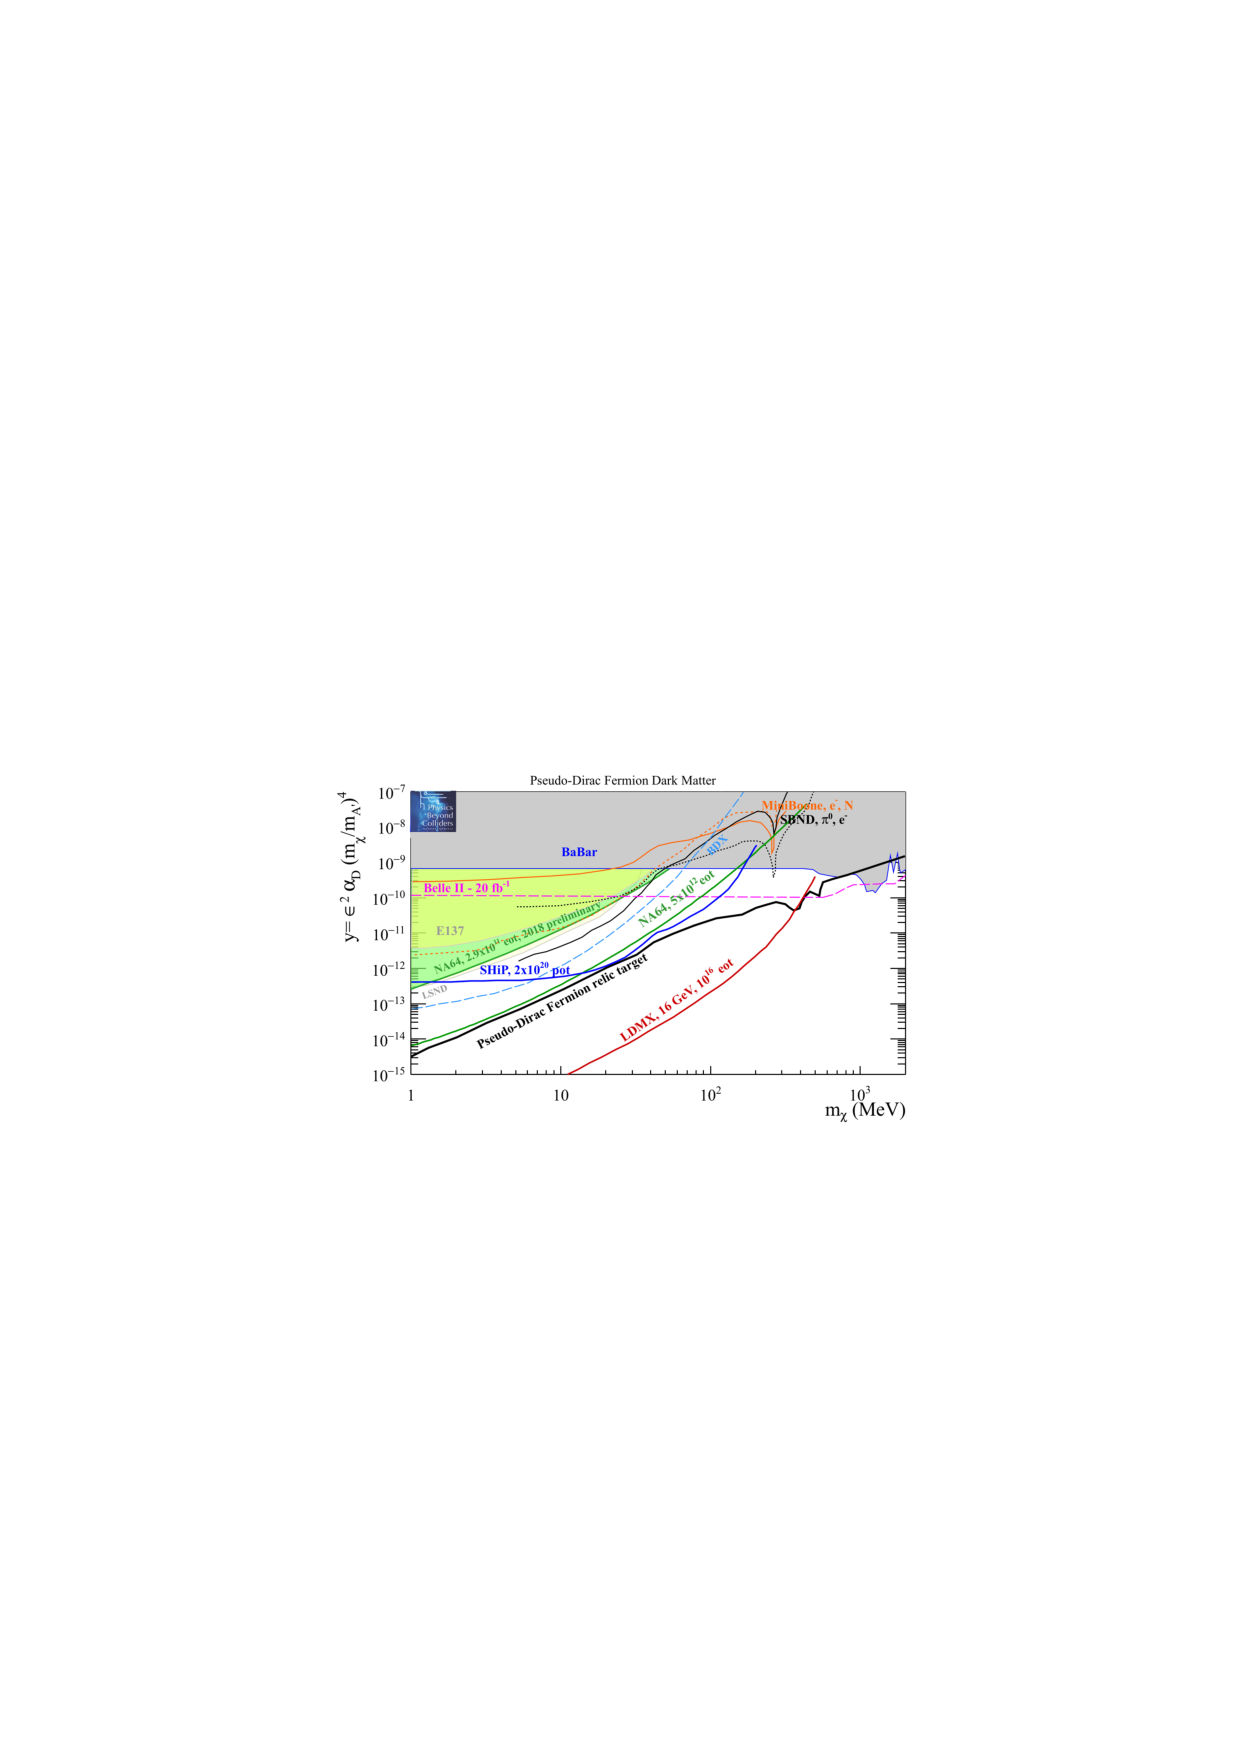
\includegraphics[width=0.8\textwidth]{Darkmatter/section3/pbc_bc2.pdf}
    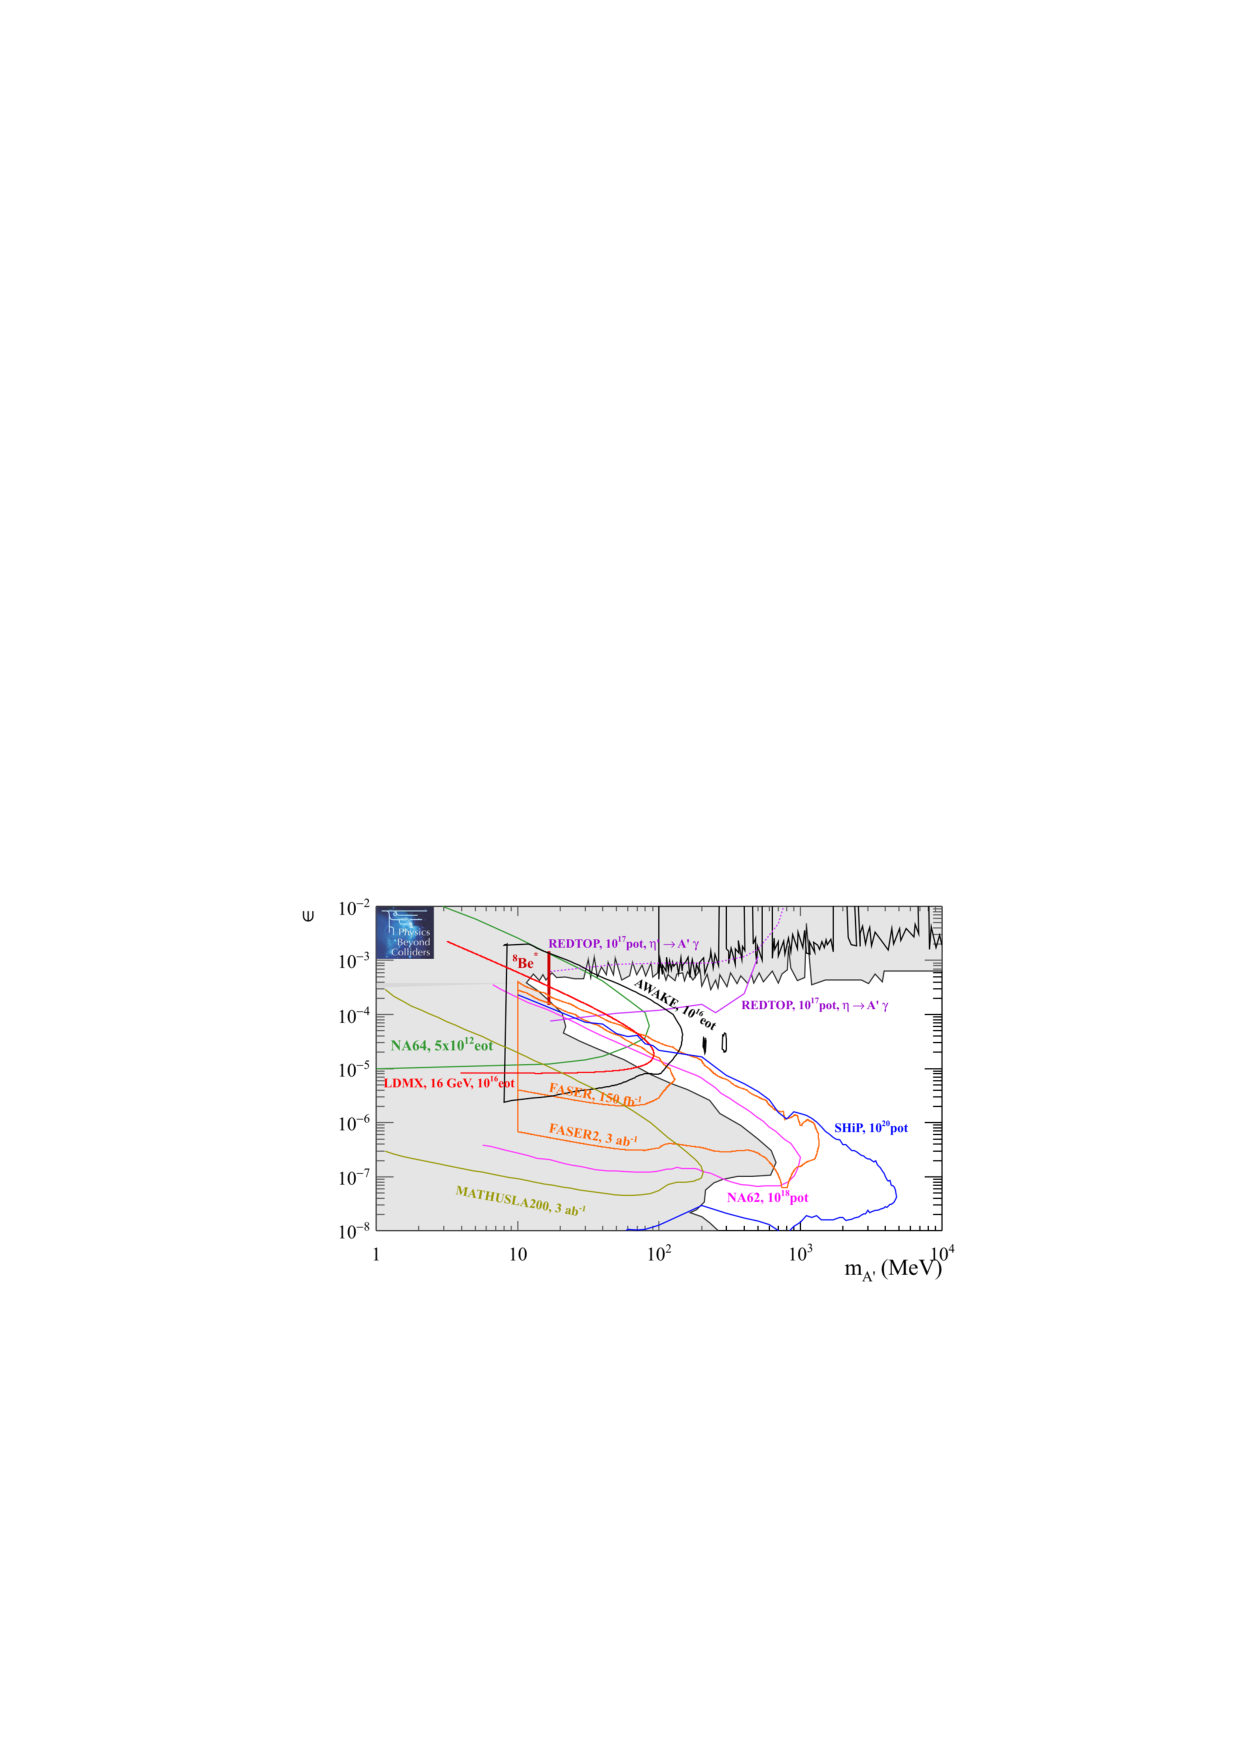
\includegraphics[width=0.8\textwidth]{Darkmatter/section3/pbc_bc1.pdf}
    \caption{Current limits and expected sensitivities of proposed experiments relevant to this section for Dark photon mediators decaying to LDM particles (top) and SM particles (bottom). These figures are taken from the PBC report~\cite{Beacham:2019nyx}. They assume a Dark coupling constant value $\alpha_D = 0.1$ and a ratio between the Dark photon ($A'$) and LDM ($\chi$) masses $m_{A'}/m_\chi = 3$.}
    \label{fig:sec3_sensitivity}
\end{figure}

%Figures~\ref{foo} to~\ref{bar} in the FIP section of the BSM chapter~\ref{blah}, show the expected sensitivities of a comprehensive list of experiments for different plausible dark sector mediators decaying into SM particles through a portal. In the majority of portals, where the mediator mass lies in the MeV to GeV range, experiments exploiting the SPS and a future Beam Dump Facility have the largest reach.

Figure~\ref{fig:sec3_LLP} shows the expected sensitivities of a comprehensive list of experiments for different plausible dark sector mediators decaying into SM particles through a portal. This includes a scalar particle with a Higgs-mixing $\sin^2 \theta$ (Higgs portal) and zero quartic self coupling (top figure), a heavy neutral lepton (HNL) mixing with active neutrinos (lepton portal) (middle figure) and an ALP pseudso-scalar that couples exclusively to photons (bottom figure). All figures are a as function of the mediator's mass and the relevant parameter defining the mediator-SM portal mixing.
In all portals, where the mediator mass lies in the MeV to GeV range, experiments exploiting the SPS and a future Beam Dump Facility have the largest reach.
%Future experiments relevant to this chapter of the briefing book are LDMX, NA64++, NA62++, SHiP and REDTOP. Further information on all of these experiments can be found in the individual submissions. 
%For both figures, the interplay with proposals that exploit the LHC interaction points (e.g MATHUSLA, Codex-b and FASER2) are also shown and are discussed in the  FIP section  of the BSM chapter{}. 
A comprehensive comparison for all portals and a discussion on the various assumptions can be found in the supplemental note accompanying this document, as well as the PBC report~\cite{Beacham:2019nyx}. 



\begin{figure}
   \centering
    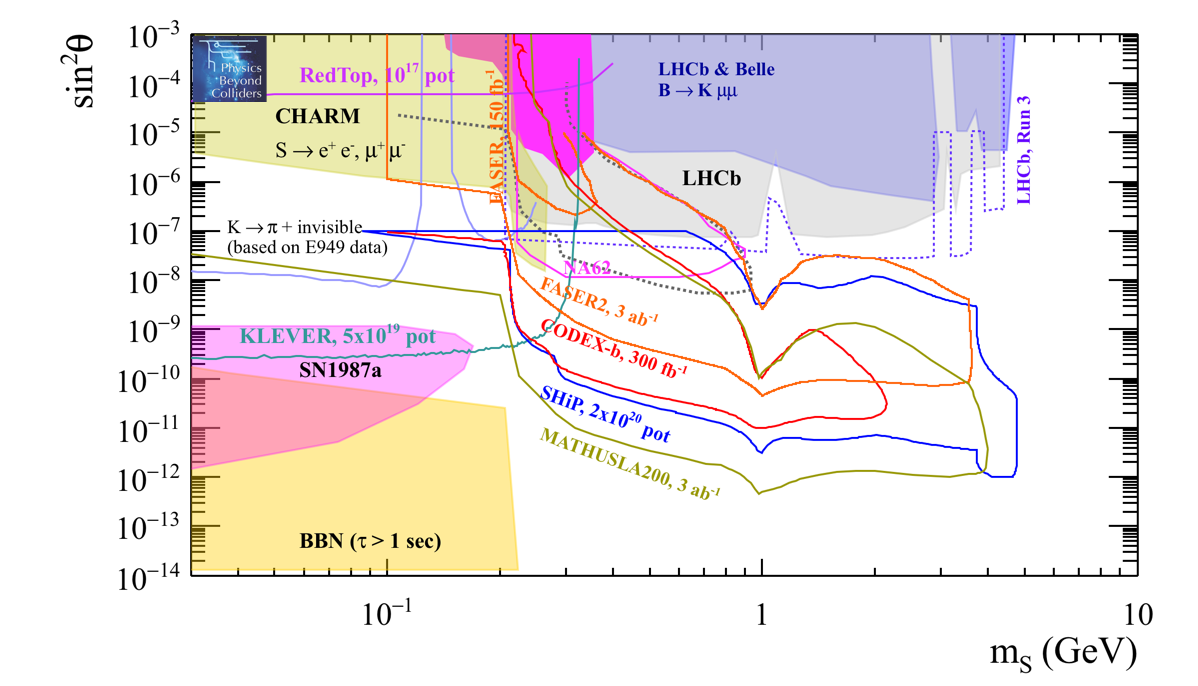
\includegraphics[width=0.7\textwidth]{Darkmatter/section3/BC4_pbc_2.png}\\
    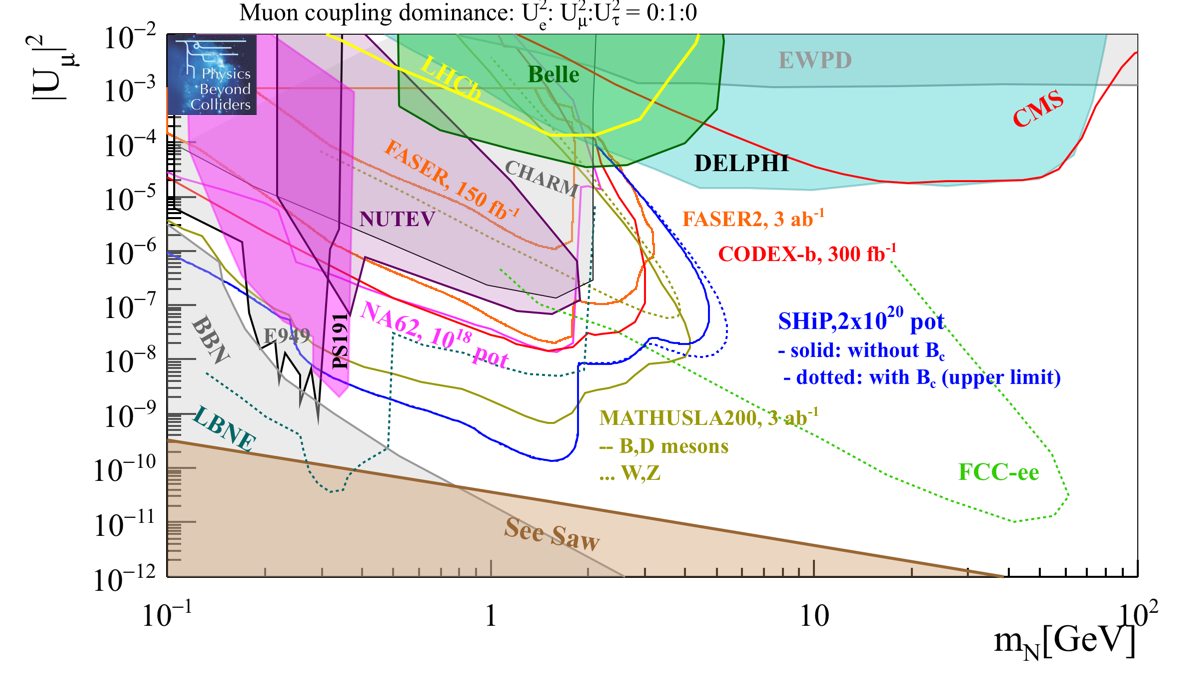
\includegraphics[width=0.7\textwidth]{Darkmatter/section3/HNL_bc7_pbc_2.png} \\
    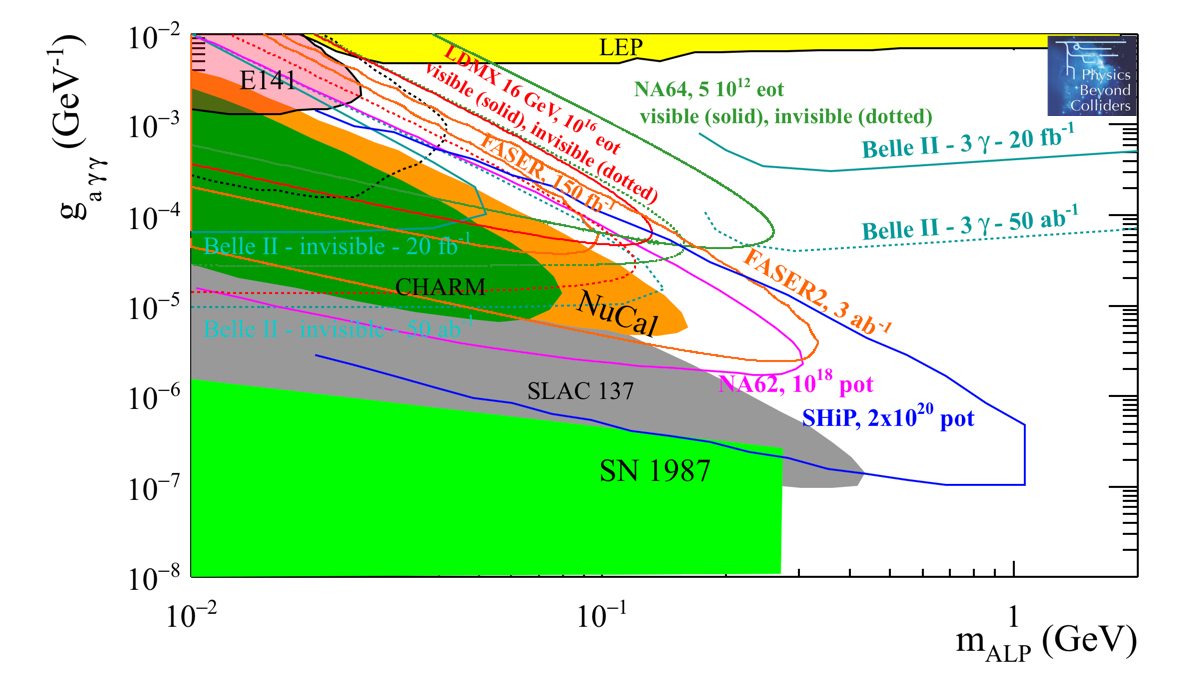
\includegraphics[width=0.7\textwidth]{Darkmatter/section3/ALPS_gg_pbc_2.png}
   \caption{ Current limits and expected sensitivities of proposed accelerator-based  experiments %relevant to this section of this briefing book
   for a scalar particle with a Higgs portal (top figure), a heavy neutral lepton (HLN)  with a neutrino portal (middle figure) and an ALP pseudsoscalar that couples exclusively to photons (bottom figure). All figures are shown as a  function of the mediator's mass and the relevant parameter defining the mediator-SM portal mixing..
   Here  the scalar is assumed to decay to SM particles though its mixing with the Higgs. 
%  The luminosities shown here reflect prospects on a 10-15 year timescale
   %for PBC projects for the dark scalar mixing with the Higgs in the mixing angle $\sin^2 \theta$ versus dark scalar mass $m_S$. (Top Right)  Current limits and projections for a heavy neutral lepton (HLN) that decays to SM particles through its lepton-portal mixing with active neutrinos. 
   The neutrino portal example   shows the mixing matrix element $|U_\mu|^2$ plotted against the HLN mass and assumes the latter HLN mixes only with muon flavored neutrinos. All plots in this figure are taken from the PBC report~\cite{Beacham:2019nyx}.% {\color{blue} Here are representative plots from the PBC report, but Kostas please make sure you're ok with this selection. --GK}
  }
   \label{fig:sec3_LLP}
\end{figure}

%\textcolor{red}{WE WOULD LIKE IF POSSIBLE TO INCLUDE THE FOLLOWING PLOTS
%\begin{itemize}
    %\item Elastic scalar LDM
   % \item Dark Scalars {\color{blue} added }
    %\item HNL  {\color{blue} added }
    %\item ALPs  {\color{blue} added }
    %\item One should probably mention other experiments such as, e.g.\\
    %Mainz (BDX, MAGIX), LNF (Padme) + US, J, Ru from (page 20)\\
    %https://indico.cern.ch/event/808335/contributions/3365155/attachments/1844071/3024799/Campana_20190515_Granada.pdf
%\end{itemize}
%}





%\subsection{Conclusions}
%  Move to chap.5 by Shoji 
%Cosmological observations of Dark Matter and the baryon asymmetry in the Universe provide overwhelming evidence of physics beyond the SM. Explorations of the energy frontier above the Electroweak scale with strong couplings to the SM have yet to provide evidence for the energy scale of new physics. There is therefore a compelling case to perform a comprehensive search for highly predictive Dark sectors in the MeV-GeV range with long-lived mediators that can address the aforementioned problems of the SM.
%Dark sectors models can provide answers to fundamental questions in particle physics, such as the origin of Dark Matter, the Baryon Asymmetry in the Universe, the origin of neutrino masses. This, coupled with a lack of a clear hint for the energy scale of new physics from the energy frontier, means that searches for Dark sectors and LDM have leading part to play in the European particle physics strategy over the next decade, with CERN playing a leading part through the proposed BDF.
%The search for a Dark sector requires  numerous experiments and techniques in order to cover the large parameter space and plethora of models. Beam dump and fixed target experiments such as SHiP, LDMX and NA64++, will perform the most sensitive and comprehensive searches in these sectors that will either discover a new sector, or will rule out models that predict thermal LDM. CERN has the opportunity to play a leading role in these searches by fully exploiting the opportunities offered by the SPS and the foreseen Beam Dump Facility.

%\subsection{The physics case}

%Although there is impressive evidence for the existence of dark matter (DM) from galactic rotation curves , gravitational lensing, the cosmic microwave background (CMB), and the matter power spectrum, these data are compatible with a wide range of DM masses between $\sim 10^{-22}$ eV -- 100 $M_\odot$. However, if the DM Standard Model (SM) interaction rate ever exceeded the Hubble expansion rate in the early universe, the DM abundance is set by the strength of the DM-SM annihilation rate independently of any assumptions about unknown cosmological epochs (e.g. inflation or baryogensis). Such a predictive, thermal origin is only compatible with DM masses between $\sim$ few keV-100 TeV, which is coincidentally in the same range of particle masses accessible at terrestrial accelerators. The upper half of this thermal window (GeV-100 TeV) contains Weakly Interacting Massive Particles (WIMPs) and is currently the focus of a broad, international effort of direct detection, indirect detection, and collider searches. However, the lighter half of this mass range (few keV - GeV) is currently underexplored and not accessible using traditional detection strategies; new techniques are necessary to comprehensively probe the predictive models in this window. 

%There are several key differences between traditional WIMPs and LDM candidates. Unlike WIMPs, which can carry electroweak charge, LDM must be neutral under all SM gauge interactions -- otherwise it would have been produced at LEP.  Furthermore, in order to achieve the observed relic density for LDM particles, such models require couplings to the SM sector that are much larger than $G_F$. This implies the existence of a new comparably light force-carrier (``mediator") between the SM and a new Dark sector. 

%Furthermore, independently of this issue, achieving the observed relic density for LDM particles requires comparably light, unstable force-carriers (``mediators") to achieve a sufficiently large annihilation rate in the early universe, with a coupling for this rate be much larger than $G_F$. 

%Thus, comprehensively probing Dark sectors and LDM in the mass range (MeV-GeV) can be organized by how these mediators couple to SM particles. Light neutral mediators can mix with neutral SM particles through so-called renormalizable portal interactions
%\begin{equation}
%F^{\mu \nu}F^\prime_{\mu \nu}~~,~~ \phi H^\dagger H ~~,~~ HLN~~,~~ \frac{im_f}{f} a \bar f \gamma^5 f
%\end{equation}
 %where $A^\prime$ is a vector mediator (``dark photon) whose field strength tensor $F_{\mu\nu}^\prime \equiv \partial_\mu A^\prime_\nu -  \partial_\nu A^\prime_\mu$ kinetically mixes with the SM photon field strength tensor and thereby acquires a coupling to the SM electromagnetic current, $\phi$ is a parity-even neutral scalar that mixes with the SM Higgs boson after electroweak symmetry breaking, $N$ is a heavy neutral lepton that mixes with active SM neutrinos. and $a$ is a parity-odd pseudoscalar (e.g. axion or axion-like particle) that couples to SM fermions $f$ through the so-called axion portal. 
 
%Dark sectors also address other unsolved problems in fundamental physics. Such sectors arise, for instance, in ``relaxion" models introduced to dynamically relax the SM higgs mass to address the electroweak hierarchy problem. Furthermore, the introduction of heavy neutral leptons can explain the origin and smallness of neutrino masses, as well as the baryon asymmetry of the universe via leptogenesis. If the heavy neutral lepton masses are at the GeV scale then they can generate this asymmetry through baryogenesis. An example of such a model is the Neutrino Minimal Standard Model~\cite{ref:XXX} ($\nuMSM$) which simultaneously addresses neutrino masses, the baryon asymmetry of the universe and provides a DM candidate. Searches for new particles and interactions have focused on masses at the Electroweak scale that are strongly coupled to the SM. However, the equally viable regime of Long lived mediators with masses below a few GeV remains largely unexplored.

 %The search strategies for these mediators depend critically on whether they decay to DM or to SM particles when produced on shell in the laboratory. 

%{\bf Mediators to LDM:} The most predictive class of LDM models involves mediators that are heavier than the LDM candidate and, therefore, decay invisibly to LDM pairs when produced on shell. Because the mediator is heavier than the DM, the only kinematically allowed annihilation process for  early-universe freeze-out involves virtual s-channel mediator exchange via DM DM > SM SM reactions. This is a particularly compelling scenario because the annihilation cross section depends on the SM-mediator coupling, which must have a minimum value in order to achieve the observed DM density. Thus, \it{invisibly decaying}  mediators feature predictive thermal DM production targets; improving experimental sensitivity to such mediators can convincingly discover or falsify a broad class of thermal DM candidates whose relic density arise from annihilation directly into SM particles in the early universe. 

%The most promising techniques for probing invisibly decaying mediators are fixed target missing energy/momentum experiments (e.g. LDMX and NA64++) which infer the production of these mediators by studying the kinematics of an electron or muon beam as it passes through an instrumented target. Since this approach derives its signal from the beam alone (and not by demanding the DM to be detected after the mediator decays) the signal rate scales as the DM-mediator coupling squared.  
%Beam dump experiments with dedicated neutrino detectors such as SHiP, can also probe invisibly decaying mediators, but this requires a two-step process: first the mediator is first produced in the target and decays promptly to DM particles. The DM daughter particles then pass through shielding to range out SM particles an then scatter off atoms inside the downstream detector, thereby depositing observable energy. However, because beam-dump expriments require {\it  both} mediator production and DM scattering in the detector, the signal rate scales as the SM-mediator coupling to the fourth power, so the reach is parametrically disfavored compared to missing energy/momentum techniques. However, this scattering technique offers complementary information by probing nucleon or quark interactions with DM.

%{\bf Mediators decaying to SM particles:} If the mediator is {\it lighter} than the DM candidate, then early universe freeze-out can proceed via DM DM > mediator mediator annihilation processes which do not depend on the SM-mediator coupling at all. However, in this regime, the mediator itself must decay to SM particles (e.g. dileptons or hadrons) and can, therefore, be detected using traditional bump-hunt techniques at colliders (e.g. B-factories or LHCb) and long-lived particle searches at beam-dump experiments with downstream detectors that search for visible energy depositions from new particles produced in upstream targets  (e.g. SHiP, NA62(++) and REDTOP). Independently to the link with thermal LDM...


%The mediator of the dark sector can decay to DM candidates (invisible decays), as well as to charged leptons and hadrons (visible decays). Different strategies are required in order to search for both types of decays.
%\begin{itemize}
 %   \item \textit{Decays to SM particles}: The mediator is produced at a proton beam dump facility. Downstream spectrometers and calorimeters reconstruct the decay of the mediator in dilepton, multihadron, lepton+hadron or di-photon final states. The rare nature of these signatures, coupled with large SM backgrounds produced in the dumping of the beam on the target, drives the experimental design. Experiments following this approach include SHiP, NA62(++)\footnote{In beam dump mode} and REDTOP.
    %%%%%%%%%%%%%%%%%%%%%%%%%%%%%%%%
  %  \item \textit{ Decays to DM particles}: There are two approaches for searching for invisible decays of the Dark sector mediator. The first relies on a fixed-target setup that performs a precise measurement of the energy/momentum of an intense electron or muon beam after its interaction with the target using precision downstream tracking and calorimetry. As this approach is independent of the final state of the mediator, it also extends the reach of searches for visible decays for mediator masses below 100~MeV. The challenge of this approach lies with the design of a high rate detector and the suppression of backgrounds produced in the interaction with the target. Experiments such as LDMX and NA64(++) are examples of this category. The second approach involves detecting the electron or nuclear recoil from the scattering of the LDM candidate with the detector. Such an 
   % approach is less sensitive to the missing energy/momentum method, however offers complementary information by probing nucleon or quark interactions with DM. The emulsion spectromemter of the SHiP experiment is an example case of this approach.
%\end{itemize}



%Models of thermal Dark Matter (DM) predict DM candidate masses ranging in the 10~keV to 100~TeV range and offer an attractive %explanation to cosmological observations with experimentally testable implications~\cite{ref:XXX}. Beam dump and fixed target %experiments will cover the MeV to GeV range, known as light thermal DM (LDM) and offer complementary reach to WIMP-like DM searches %described in Sec.~\ref{sec:XXX}. 

%In order to obtain the correct relic abundance, LDM models require couplings to the SM sector that are larger than $G_F$. This implies %the existence of a new force-carrier (mediator) between the SM and a new Dark sector where the DM candidate is one of the particles of %this new sector. The lowest dimensional renormalisable portals between the SM and the Dark sector are given by: \textcolor{red}{List %portals and their interactions}

%\subsection{Experimental requirements}
%As the mediators of the Dark sector couple weakly to the SM, facilities with high energy and intensity beams impinging on dense targets are essential in order to maximise the experimental sensitivity to such models. Facilities at CERN's SPS or SLAC's LCLS-II, will have unprecedented sensitivity to a wide range of Dark sector models and offer unique opportunities to explore large portions of the relevant parameter space.

%The interaction of the beam with the target results in the production of Dark sector mediators through multiple mechanisms. For fixed-target type experiments searching for invisible decays of the mediator through the missing energy/momentum technique (see below), the dominant production mechanism is through Bremsstrahlung. In experiments where the beam is dumped on a target (beam dump), additional mechanisms are available such as Drell-Yan and decays of hadrons produced in the collision of the beam with the target. Decays of charm and beauty hadrons provide additional sensitivity to mediators with masses in the multi-GeV mass domain. 

%The ability to categorically determine that a potential signal is not an instrumental effect or an unaccounted background, is paramount in searches for rare signatures. Detectors need to have redundant systems for suppressing backgrounds and be able to define control regions in order to check the level of agreement with expected background rates. In addition, the ability to provide independent confirmation that a potential signal originated from the target, by reconstructing the momenta of the decay products of the mediator (or otherwise) gives confidence on the validity of an HS signature. 

%A comprehensive search for Hidden Sectors must look for both types of final states. In the advent of a Dark sector signature decaying to visible final states, experiments must be able to provide precise information on the mass and couplings for a range fully- and partially-reconstructed final states, shedding light on the type of new physics observed. For instance, if a signal is seen in the $\mu^+\mu^-$ final state but not in $\mu\pi$, with a commensurate signature seen in the di-photon, final state, this would indicate the existence of a (Pseudo-)Scalar mediator rather than a dark photon or heavy neutral lepton.




%\subsection{Experimental overview}

%\subsubsection{Invisible decays}\\

%{\bf \noindent Current constraints}\\
%\noindent The latest constraints on Light DM come from...\\

%{\bf \noindent Future experiments}\\

%\subsubsection{Visible decays}\\

%{\bf \noindent Current constraints}\\\\

%\noindent The latest constraints on visible decays of Dark sector mediators come from...
%\\

%\subsubsection{Recent experiments}
%NA62, NA64, MiniBooNe, HPS, APEX

%\subsubsection{Future directions}

%Extensive studies have been performed for a new general purpose beam dump facility (BDF) at the CERN SPS accelerator aimed at exploring the domain of Dark sector models and performing measurements involving $\tau$ neutrinos Lepton Flavour Violating decays of $\tau$ leptons. The high intensity of the SPS 400~GeV beam allows to probe a wide variety of models containing long-lived exotic particles with masses below $\mathcal{O}(10)$GeV. A new beamline, target complex and experimental hall at the North Area of CERN is foreseen, to deliver $4\times10^{13}$ protons on target during 1~second spills using slow extraction of the beam. The Search for Hidden Particles (SHiP) experiment is a major use case for the BDF. It relies on a magnetic ``muon shield'', veto systems and fast timing detectors to suppress the backgrounds to zero over its 5 years of operation where it will collect $2\times10^{20}$ protons on target. It is equipped with a dual spectrometer system: an emulsion spectrometer to detect LDM candidates produced from the initial interaction as well as to perform $\nu_\tau$ physics; and a decay vessel with a spectrometer followed by calorimeter and muon systems for $e/\mu/h$ separation. The SHiP collaboration recently completed a Comprehensive Design Study demonstrating good control over the slow extraction and losses of the SPS beam, the design of the target complex and the performance of the active muon shield. A Conceptual Design Report foreseen for end of EPPSU at which point the project will be mature enough for an implementation decision to be made. The first physics run is expected to take place during Run4 of the LHC, starting in 2027.


%It has been proposed to use the SPS to accelerate and deliver 16~GeV electrons (eSPS) for the LDMX experiment using slow extraction at a rate of $10^{16}$ electrons per year. This would be achieved by leveraging CLIC technology to  accelerate electrons to 3.5~GeV before injecting into the eSPS. Initial studies demonstrate that such an operation is feasible, however it would require reserving 30\% of the SPS duty cycle towards this project. 
%\textcolor{red}{A few words about LCLS-II???}

%\textcolor{red}{Hard sell... need to tone down and shorten and also add LDM scattering:}\\
%The Search for Hidden Particles (SHiP) experiment at the SPS BDF will search for all the aforementioned Dark sector portals using $2\times10^{20}$ protons on target delivered by the SPS during its five years of planned operation. This will be achieved through two main points. Firstly, using the copious amounts of charm, beauty, $\tau$ leptons and photons produced in an interaction of the intense SPS beam with the SHiP target which in turn can produce Dark sector particles. Secondly, by reducing the background to zero over the experiment lifetime through the combination of a magnetic ``muon  shield'' to sweep away muons from reaching the detector acceptance, veto systems surrounding the detector, timing coincidence through a dedicated fast timing detector, and a magnetic spectrometer within the decay volume. The SHiP experiment 
%enables the unambiguous determination of the origin of a fully reconstructed Hidden Sector candidate produced in the proton collision with no assumptions. This is achieved through the dedicated spectrometer positioned within the decay volume of the detector. This spectrometer also allows the determination of the mass of a Hidden Sector particle with a resolution of 15~MeV. Calorimeter and muon systems located downstream of the spectrometer will be able to identify the type of particles involved in the decay of a Hidden Sector signature ($e$/$\mu$/hadron separation). The SHiP collaboration recently completed a Comprehensive Design Study done demonstrating good control over the slow extraction and losses of the SPS beam, the design of the target complex and the performance of the active $\mu$ shield. A Conceptual Design Report foreseen for end of EPPSU at which point the project will be mature enough for an implementation decision to be made.

%\textcolor{red}{Add something about LDMX}\\

%\textcolor{red}{Say something about a two stage approach ie SLAC then CERN}\\

%\subsubsection{Interplay with other communities}
%\textcolor{red}{Say something about links with Collider searches, Flavour experiments, Direct DM detection}

%\subsection{Conclusions}
%Cosmological observations of Dark Matter and the baryon asymmetry in the Universe provide overwhelming evidence of physics beyond the SM. Explorations of the energy frontier above the Electroweak scale with strong couplings to the SM have yet to provide evidence for the energy scale of new physics. There is therefore a compelling case to perform a comprehenseive search for higly predictive Dark sectors in the MeV-GeV range with long-lived mediators that can address the aforementioned problems of the SM.
%Dark sectors models can provide answers to fundumental questions in particle physics, such as the origin of Dark Matter, the Baryon Asymmetry in the Universe, the origin of neutrino masses. This, coupled with a lack of a clear hint for the energy scale of new physics from the energy frontier, means that searches for Dark sectors and LDM have leading part to play in the European particle physics strategy over the next decade, with CERN playing a leading part through the proposed BDF. 
%Beam dump and fixed target experiments such as SHiP, NA62++, LDMX and NA64++, will perform the most sensitive and comprehensive searches in these sectors that will either discover a new sector, or will rule out models that predict thermal LDM. We recommend that CERN plays a leading role in these searches by fully exploiting the opportunities offered by the SPS and the planned Beam Dump Facility.


\subsection{Complementarity with direct and indirect detection}

In addition to the accelerator program outlined here, there has been considerable progress developing new techniques for low-threshold direct detection searches, typically involving novel targets including electrons \cite{Essig:2011nj}, semiconductors~\cite{Essig:2015cda}, graphene~\cite{Hochberg:2016ntt}, superconductors \cite{Hochberg:2015fth}, and several others. These techniques are very promising if DM scatters in a velocity-independent, elastic manner. Currently running experiments, including SENSEI \cite{Tiffenberg:2017aac}, DAMIC \cite{Aguilar-Arevalo:2019wdi}, and CRESST \cite{Petricca:2017zdp} 
%and the near-future NEWAGE 
will reach the scalar LDM thermal sensitivity target for masses below ~ 100 MeV, as shown in the supporting document. However, if DM scatters inelastically or with velocity dependence in the non-relativistic limit, these experiments typically do not improve upon existing limits for these models and accelerator searches are essential for reaching important experimental milestones.

Beam dump experiments will furthermore probe dark matter models with light $\sim$MeV mediators, which, e.g., can induce gamma-ray emission from the Sun, observable with Fermi LAT and water Cherenkov detectors like HAWC~\cite{Arina2018-gl}.  More generally, operators responsible for the annihilation/decay of sub-GeV dark matter particles, which can be explored with proposed future MeV missions like AMEGO~\cite{Moiseev2018-kg}, can potentially lead to observable signatures at beam dump experiments \cite{Kumar2018-be}.  Upcoming beam dump experiments like SHiP or NA62++ can probe the two heavier right-handed neutrinos predicted by the $\nu$MSM models~\cite{Beacham2019-os}, which can explain the observed 3.5 keV feature in X-ray data in terms of sterile neutrino dark matter~\cite{Bulbul2014-on, Boyarsky2014-gy}.

\end{document}

